\subsection{Robot Prototype}
During data collection, several kinematic limits (shown in Table \ref{tab:physical_limits}) to the prototype became obvious. Maximum tested speeds under contraction reached \SI{0.2}{m/s} while maximum speeds under extension reached \SI{1.0}{m/s}. 

\begin{table}[h]
    \centering   
    \caption{Prototype physical limits}
    \begin{tabular}{p{0.35\linewidth} | p{0.2\linewidth}}
        \textbf{Limit} & \textbf{Value} \\
        \hline
        Top contraction speed & \SI{0.2}{m/s} \\
        Top extension speed & \SI{1.0}{m/s} \\
        Maximum curvature & \SI{7.39}{m^{-1}} \\
        Failure rates & $\mu =$ \SI{83.2}{min}\newline$\sigma =$ \SI{48.9}{min}
    \end{tabular}
    \label{tab:physical_limits}
\end{table}

\paragraph{The primary failure modes} of this prototype are tendons breaking and the tendon spindle snapping. During data collection, the robot had four critical failures where a piece on the physical system broke. Twice the tendons snapped and twice the spindle sheared (Figure \ref{fig:sheared_spindle}). 

\begin{figure}[h]
    \centering
    \makebox[\textwidth][c]{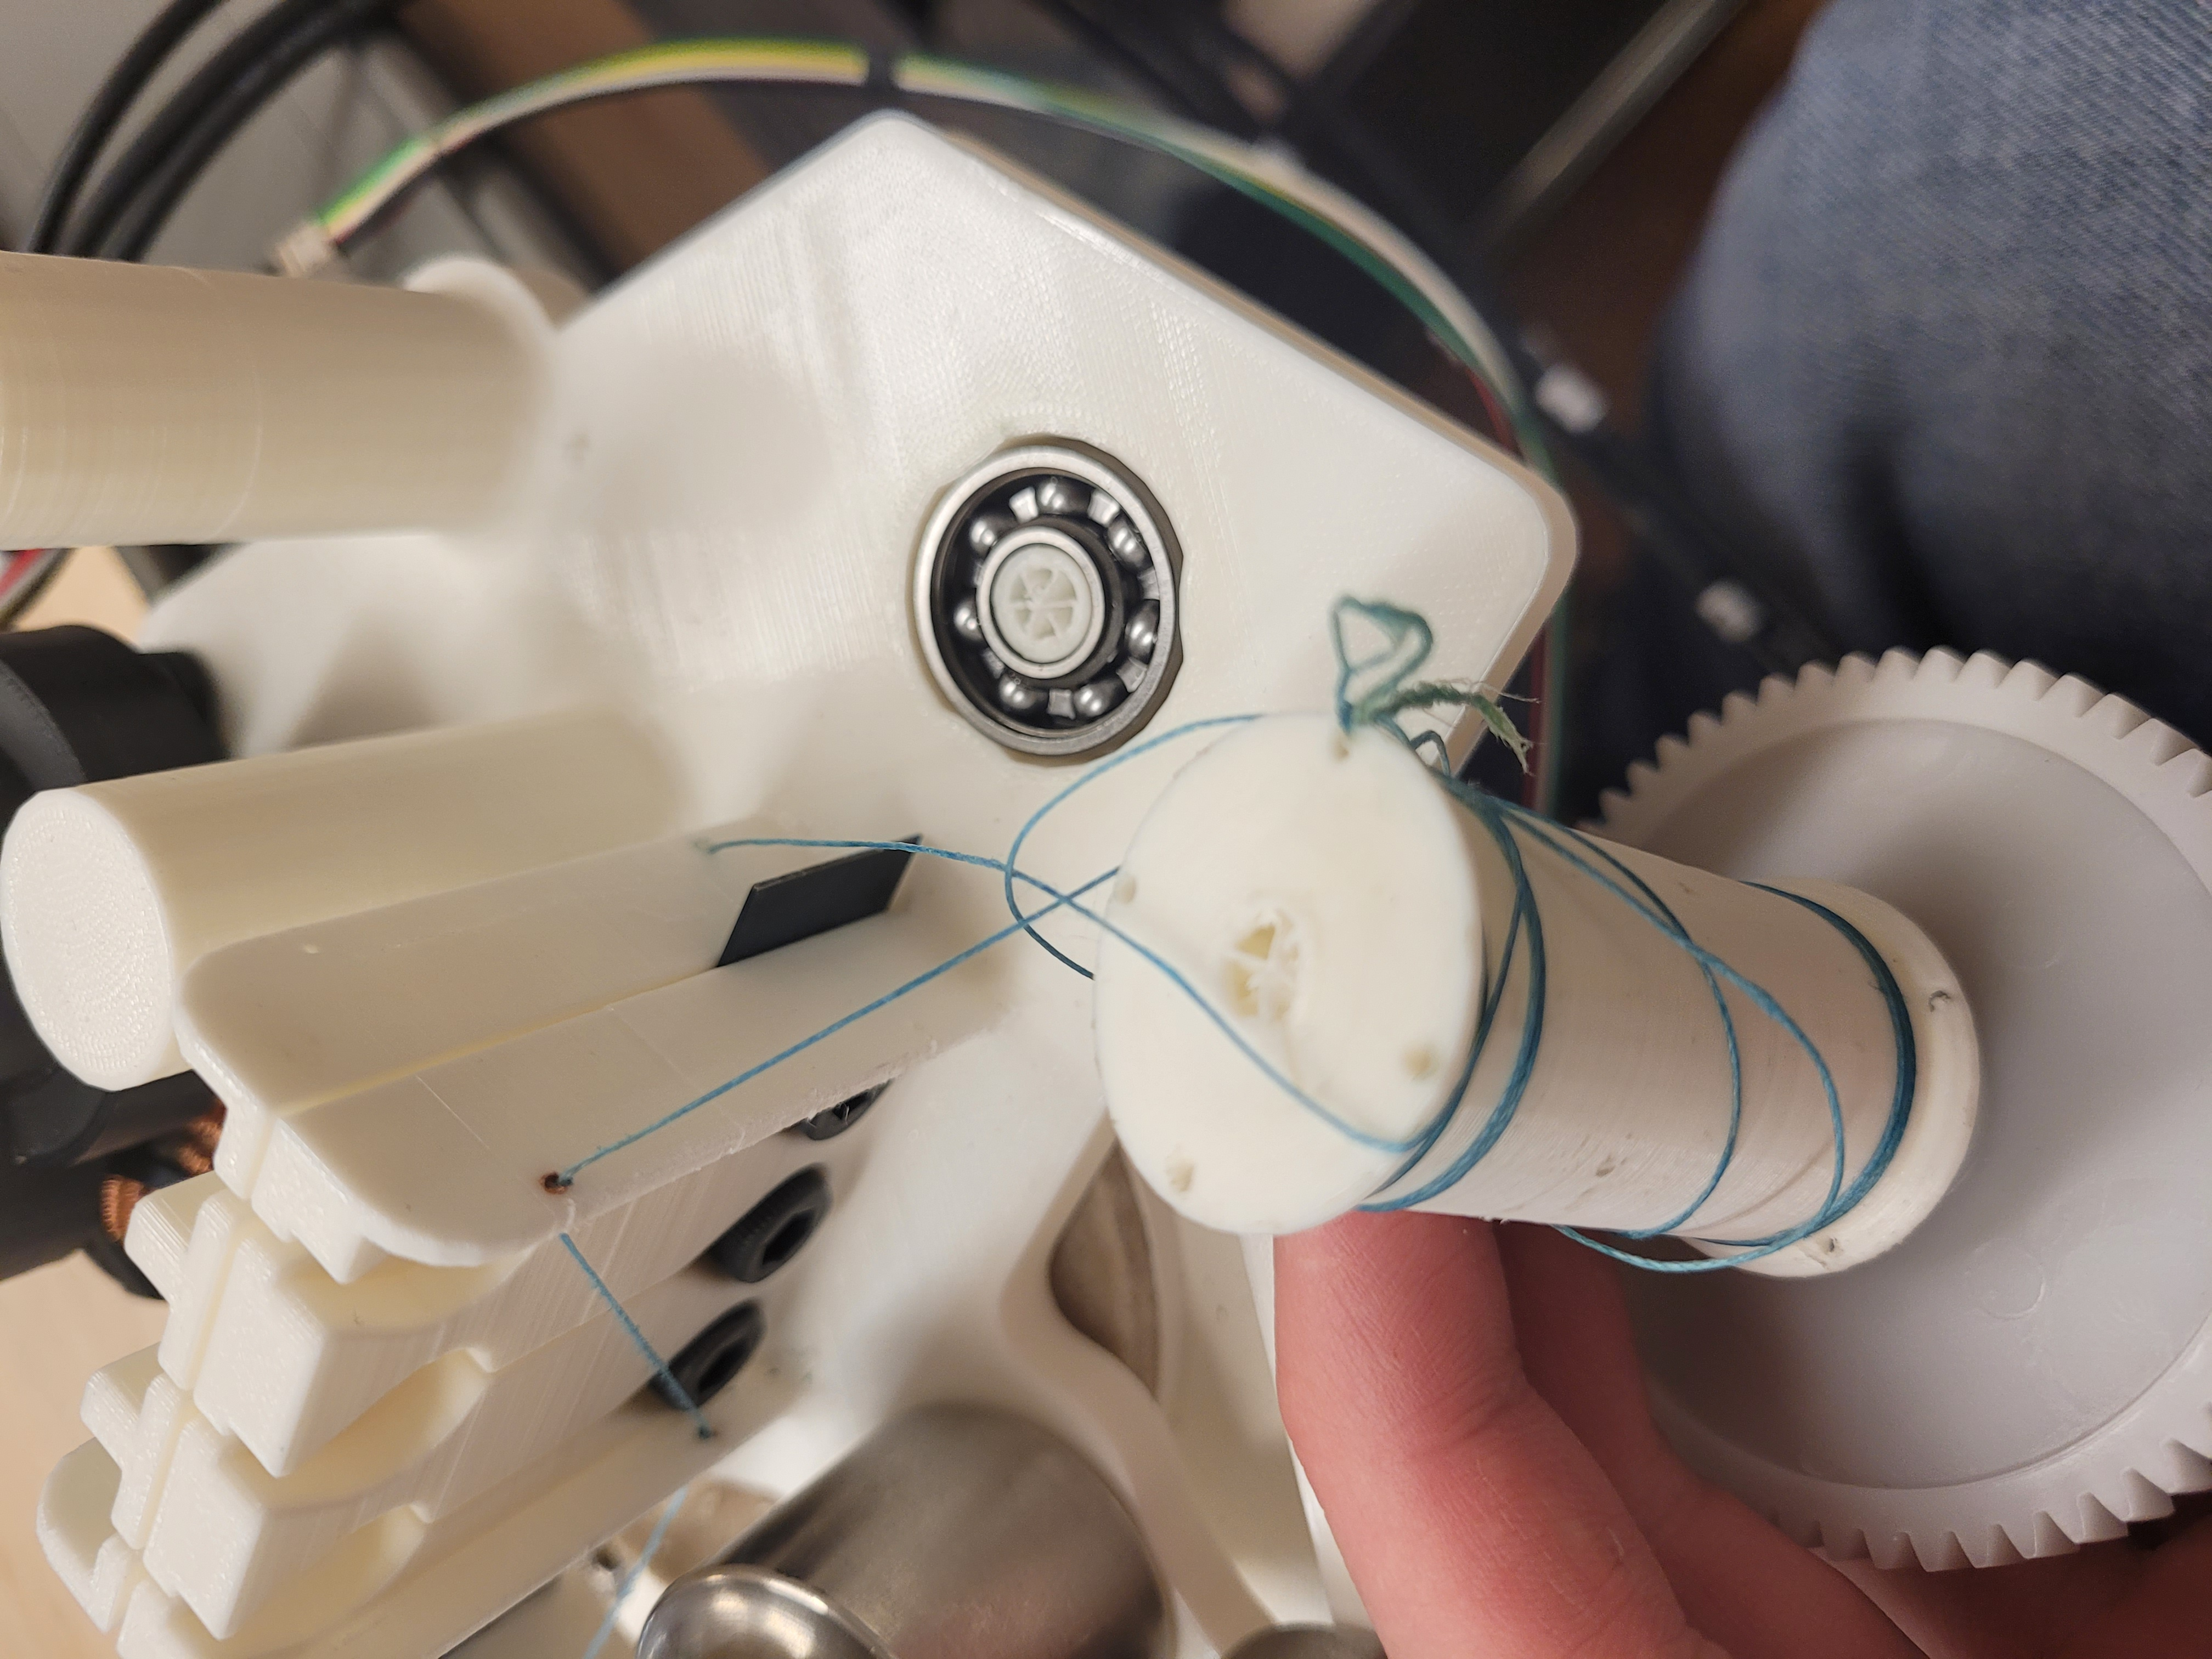
\includegraphics[width=0.8\textwidth]{images/sheared_spindle.jpg}}
    \caption{Tendon spindle shear failure}
    \label{fig:sheared_spindle}
\end{figure}